\section{Foundations}
\subsection{Derivation of EOM of many body system}
Hamiltonian of single atom dispersively coupled to single cavity mode by a running-wave laser drive 
\begin{equation}
	\hat{H}_{SP} = \frac{\hat{p}^2}{2M}- \hbar \omega_z \hat{F}_z + \hbar q \hat{F}^2_z + \hbar \omega_c \hat{a}^\dag \hat{a}-i \frac{\alpha_\nu}{2F}\left [ \bm{\hat{E}}^{(+)} \cross \bm{\hat{E}}^{(-)} \right ] \cdot \bm{\hat{F}} .
\end{equation}
Operator $\hat{a}$ creates photon in z-polarized cavity mode of frequency $\omega_c$. Second and third term are Zeeman splittings. $\bm{\hat{F}}$ is spin operator.
\begin{figure}[h!]
	\centering
	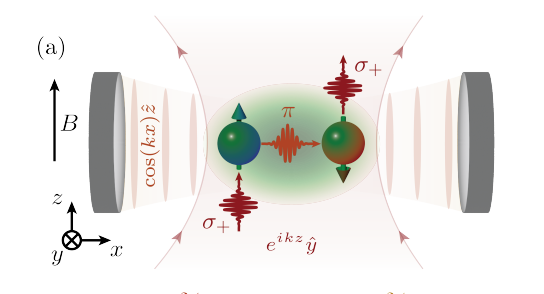
\includegraphics[width=1\linewidth]{Images/scetch_pair_production.png}
	\caption{Pair production}
	\label{fig:scetch_pair_production}
\end{figure}
\\ \break
Second quantization 
\\ \break
Spinor field operator \text{RHS "5-mode-expansion" doesnt contain second summand}
\begin{equation}
	\hat{\Psi} (\bm{x}) = \left (
	\begin{matrix}
		\frac{k}{\sqrt{2}\pi} \cos(kx) ( e^{ikz}\hat{c}_{+k,+1} + e^{-ikz} \hat{c}_{-k,+1})
		\\
		\frac{k}{2 \pi}\hat{c}_{0,0} + \frac{\sqrt{2}k}{\sqrt{3}\pi} \cos^2(kx)\hat{c}_{\pm2k_x,0}
		\\
		\frac{k}{\sqrt{2}\pi} \cos(kx) ( e^{-ikz}\hat{c}_{-k,-1} + e^{ikz} \hat{c}_{+k,-1})
	\end{matrix} \right)
	= \left (
	\begin{matrix}
		\hat{c}_{+1,+k} \psi_{+1,+k} + \hat{c}_{+1,-k} \psi_{+1,-k}
		\\
		\hat{c}_{0,0}\psi_{0,0} 
		\\
		\hat{c}_{-1,k} \psi_{-1,+k} + \hat{c}_{-1,-k}\psi_{-1,-k}
	\end{matrix}
	\right)
\end{equation}
Where the respective functions have to be normed
\begin{equation}
	\int_{\frac{-\pi}{k}}^{\frac{\pi}{k}}  \psi^*_{+1,+k} \psi_{+1,+k} dz dx = 1
\end{equation}(c.f. 2010 Dicke paper)
\begin{equation}
	\Psi = \left( \begin{matrix}
		\Psi_{+1}
		\\
		\Psi_0
		\\
		\Psi_{-1}
	\end{matrix}\right)
\end{equation}
Next we find an effective many body hamiltonian.
\begin{equation}
	H_{SP} = H_L + H_{AT} + H_{INT}
\end{equation}
Where $H_{AT}$ contains $F_z$ and $H_{INT}$ contains $F_+, F_-$.
\begin{equation}
	H_{MB} = H_L + \int \hat{\Psi}^\dag(\hat{x}) ( H_{AT} + H_{INT}) \hat{\Psi}(\hat{x}) \hat{dx}
\end{equation}

e.g. 
\begin{equation}
	F_z = \left( 
	\begin{matrix}
		+1 && 0 && 0
		\\
		0 && 0 && 0 
		\\ 
		0 && 0 && -1
	\end{matrix}
	\right) 
\end{equation}
\begin{equation}
	F_+ =\sqrt{2} \left( 
	\begin{matrix}
		0 && 1 && 0
		\\
		0 && 0 && 1 
		\\ 
		0 && 0 && 0
	\end{matrix}
	\right) 
\end{equation}
This calculation is done in Rodrigos "Full derivation Hamiltonian" handwritten pdf. We do adiabatic elimination with effective operators and apply the rotating wave approximation. 
We obtain the effective many-body Hamiltonian
\begin{equation}\label{eq:fou_effective_many_body_hamiltonian}
	H = H_0 + H_+ + H_-
\end{equation}
with e.g.
\begin{equation}
	H_+ = \hbar \chi_+ (2 \hat{c}^\dag_{-k,-1} \hat{c}^\dag_{+k,+1}\hat{c}_0 \hat{c}_0+ \hat{c}^\dag_0 \hat{c}_{+k,+1}\hat{c}^\dag_{+k,+1}\hat{c}_0 + \hat{c}^\dag_{-k,-1}\hat{c}_0\hat{c}_0^\dag \hat{c}_{-k,-1} + h.c.)
\end{equation}
\subsection{Further info to experiment: (rodrigo thesis p.103)}
drive is operated in limit of large two-poton  detunings
\begin{equation}
	|\delta_\pm| \gg \kappa
\end{equation}
\begin{equation}
	\delta_\pm = \delta_c \pm \omega_z = (\omega_d \pm \omega_z) - \omega_c
\end{equation}
We absorb drive photon, and go from 
\begin{equation}
	\ket{0}_0 \rightarrow \ket{+k}_+1
\end{equation}
thus we need a energy conserving cavity photon with freq $\approx \omega_d - \omega_z$. (or $+\omega_z$?) Here we can still ignore the kinetic energy $\sim k$ of the atom since this energy is much smaller than $\kappa$.
\\ 
Parametric amplification of pair production
\\
look at \ref{eq:fou_effective_many_body_hamiltonian} + assume mode $\ket{0}_0$ undepleted throughout the dynamics i.e. occupied by N atoms. set $\hat{c}_0$ = $\sqrt{N}$ and obtain
\begin{equation}
	\hat{H}_{eff} = \hat{H}^+_{eff} + \hat{H}^-_{eff}
\end{equation}
with 
\begin{equation}
	\hat{H}^\pm_{eff} = \hbar (\omega_0 + 4 N \chi_\pm)(\hat{K}_{z,\pm}-1/2) + 4 \hbar N \chi_\pm \hat{K}_{x,\pm}
\end{equation}
Look at linear equations of motion
\begin{equation}\label{eq:fou_time_development_linear_K}
	\dt{}\left( 
	\begin{matrix}
		\hat{K}_{x,\pm}
		\\
		....y
		\\
		...z
	\end{matrix}\right) = \bm{M}_\pm 
	\left( \begin{matrix}
	\hat{K}_{x,\pm}
	\\
	....y
	\\
	...z
	\end{matrix}\right)	
\end{equation}
with three non-degenerate complex eigenvalues
\begin{align}
	\lambda_{1,\pm} = 0 
	\\
	\lambda_{2,\pm} = \sqrt{-\omega_0(\omega_0 + 8 N \chi_\pm)} \eqcolon + \lambda_\pm
	\\
	\lambda_{3,\pm} = - \sqrt{- \omega_0 (\omega_0+8N \chi_\pm)}
\end{align}
We also have
\begin{equation}\label{eq:fou_time_development_particle_number}
	\langle N_{p,\pm} \rangle = \frac{1}{2} (\langle c_{1,\pm}^\dag c_{1,\pm} \rangle + \langle c_{-1,\mp}^\dag c_{-1,\mp}\rangle ) \approx \langle K_{z,\pm} \rangle - \frac{1}{2} \approx A\cosh(\lambda_\pm t) + \text(const)
\end{equation}
To conclude: we see that we have eigenvectors of M. Those are perpendicular, since the eigenvalues are different. The time development of those is given by \ref{eq:fou_time_development_linear_K}. Thus, its either phase oszillation for a complex eigenvalue or exponential growth for a real eigenvalue. \ref{eq:fou_time_development_particle_number} looks at the expectation value of the occupation of the modes that are not $\ket{0}_0$ (occupation of pairs). we see that the time development of those depends on $ \langle K_{z,\pm} \rangle$, therefore on the eigenvectors of M, therefore on the eigenvalues of M. We see, that for a real $\lambda_\pm$ the occuopation of those modes get macroscopic. So we say that for a critical coupling a second order phase transition occurs (lambda get real) featuring pairs. this fast change of coupling is called quench (faster that any period of oscillations happening in system e.g. $1/\omega_0$). 
\\
Note: if the number of pairs gets high, the undepleted approximation doesnt hold anymore. thus this equations can just predict the inital growth of pairs. (later there is saturation)
\\
quench: the system jumps from one set of eigenstates to another set of eigenstates. before system was in single eigenstate, after quench it is superposition of different eigenstates $\rightarrow$ oscillation of those. this cant be expressed analytically, thus calculations are done numerically. 
\begin{figure}[h!]
	\centering
	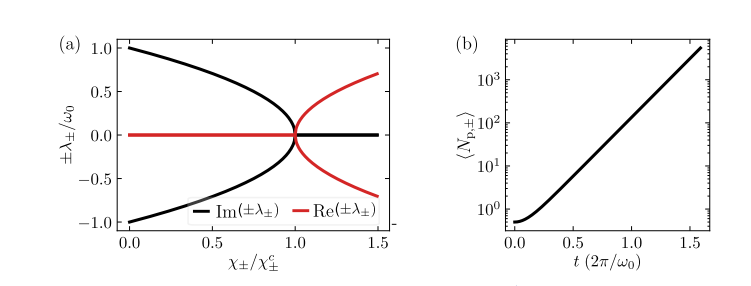
\includegraphics[width=1\linewidth]{Images/scetch_quench_parametric_amplification.png}
	\caption{Parametric amplification}
	\label{fig:scetch_quench_parametric_amplification}
\end{figure}
\subsection{The energy scales}
not sure, whether all plus /minus are choosen correctly in scetch, but the scheme looks approximately like this:  
\begin{figure}[h!]
	\centering
	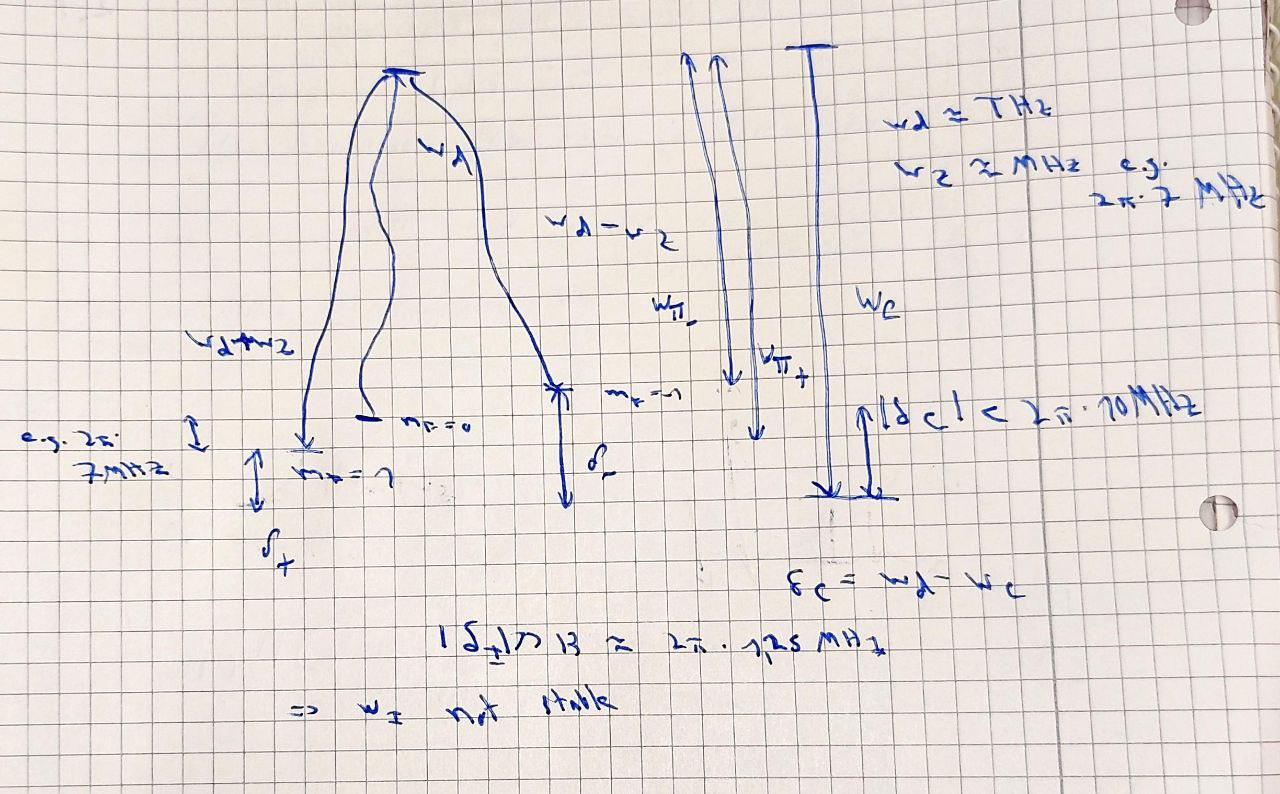
\includegraphics[width=1\linewidth]{Images/energy_scetch.jpeg}
	\caption{Energy scetch}
	\label{fig:energy_scales}
\end{figure}
We start in the Rb87 5 2 S1/2 F=1 (F... total angular momentum) fine structure) (https://steck.us/alkalidata/rubidium87numbers.1.6.pdf). We send light $\omega_d$ with $\lambda 790.02nm$. The transition to the  5 2 P3/2 (D2 transition) is around 980nm the transition to 5 2 Pb1/2 (D1) is around 995nm. thus, we are blue detuned with D1 and red detuned with D2 (check whether its not other way around)(one of the wavelength in Rb is wrong). This is called Tune out-wavelength. Even though it is not exactly the middle it is the effective middle. So the scalar polarization $\alpha_s$ is zero and there is no dipole potential trapping the atom. We are off resonant by THz and therefore wont reach any population in the 5 2 P levels (dispersive regime). N I S H A N T  Dogra phdthesis ch3.1. explains this detailed. 
\\
the energy of the $\pi$ photon is $\omega_\pm$ = $\omega_d \pm w_z$. So something like Thz $\pm$ e.g. $\omega_z = 2\pi 7 $MHz.
\\
The cavity wavelength is chosen to be similar to the drive wavelength: $|\delta_c| = |\omega_d - \omega_c| < 2\pi 10$MHz. But the cavity wavelength is off resonant to the $\pi$ photon wavelength if we compare this detuning $\delta_\pm$ (= diff $\omega_\pm$ and $\omega_c$) with the cavity loss $\kappa$. $|\delta_\pm | \gg \kappa$
\\
From somewhere we get
\begin{equation}\label{eq:fou_coupling}
	\chi_\pm = \eta^2 \frac{\delta_\pm}{\delta_\pm^2 + \kappa^2}
\end{equation}
and
\begin{equation}
	\gamma_\pm = \frac{\eta^2 \kappa}{\delta_\pm^2 + \kappa^2}.
\end{equation}
\begin{equation}
	\eta \sim \alpha_\nu E_d E_0
\end{equation}
where $\alpha_\nu$ vectorial polarisierbarkeit, $E_d$ intensity of drive, $E_0$ electric field of vacuum of cavity mode =$\rangle$ given by geometry. \ref{eq:fou_coupling} shows, that for high $\omega_z$ the first atom will be most likely in state $\ket{+k,+1}$. This is because high $\omega_z$ implies high $| \delta_- |$ and small $| \delta_+ |$ which leads to a stronger coupling for the + channel. 
\\
Experimentally we can change $\delta_c$ and $\omega_z$.  
\\ 
 how is k defined? $k=k_z$?. own consideration: let $\omega_c$ = $\omega_d$ + x, where x is order of MHz. We get by Taylor
 \begin{equation}
 	\lambda_c = \frac{c}{\omega_d + x} = \frac{c}{\omega_d}- x \frac{c}{\omega_d^2} + O(x^2) \approx \frac{c}{\omega_d} = \lambda_d.
 \end{equation}
Thats the reason, why we use for python just one single wavelength $\lambda_M$. So we can conclude that $k_z \approx k_x$ (=k, right?). 
 \\
 With this result we look at the energies of different states: 
 \begin{equation}
 	\psi_{\pm 2 k, 0} \approx N \cos(2kx) \otimes \ket{m=0}
 \end{equation}
 and therefore
 \begin{equation}
 	E_{rec} = \frac{\hbar^2 (2k)^2}{2m} = \hbar 4 \omega_{rec}
 \end{equation}
 with 
 \begin{equation}
 	\omega_{rec} =  \frac{\hbar k^2}{2m}
 \end{equation}
 (check formulas, rodrigo gave them to me.).
 \\
 We also get
 \begin{equation}
 	\psi_{+k,+1} \approx N \cos(kx)e^{ikz}.
 \end{equation}
\begin{align}
	E_{kin} &= \int \psi_{+k,+1} \hbar \left ( \frac{\partial_x^2 + \partial_y^2}{2m} \right) \psi_{+k,+1} dx dz
	\\
	& =\frac{\hbar k_x^2 + \hbar k_z^2}{2m} = 2 \omega_{rec}.
\end{align}
So if we consider the creation of a single pair, we get that this pair has energy 
\begin{equation}
	\omega_0 = 2q + 4 \omega_{rec}
\end{equation} 
in comparison to the to atoms in the BEC. The first order zeeman splitting cancelled out such that only the 2nd order Zeeman splitting q and the kinetic energy $\omega_{rec}$ contribute. (check with rodrigo, whether this is correct understanding. for this understanding we dont need to consider rotating frame.). We see that for small q the $\ket{\pm 2k,0}$ and $\ket{+k,+1}$ modes have the same energy scale. 
\\
Derivation of recoil energy:
\begin{equation}
	E_{rec} = \frac{p_{rec}^2}{2m} = \frac{\hbar^2 k^2}{2m} = \frac{\hbar^2 4 \pi^2}{2 m \lambda^2} = \hbar \omega_{rec}.
\end{equation}
\subsection{Number squeezing}
Following (thesis Finger)
\\
Introduce imbalance operator
\begin{equation}
	\hat{J}_z = \frac{1}{2} (\hat{N}_{+1}- \hat{N}_{-1})
\end{equation}
where $\hat{N}_{+1} = \hat{c}_{+k,+1}^\dag \hat{c}_{+k,+1}$ and $\hat{N}_{-1} = \hat{c}_{-k,-1}^\dag \hat{c}_{-k,-1}$. 
We introduce 
\begin{equation}
	\xi_N^2 = \frac{4 \sigma^2(\hat{J}_z)}{N}
\end{equation}
where $\sigma^2(\hat{J}_z)$ is variance of imbalance operator. Normalize to the squeezing parameter $\xi_{N,coh}^2$ of uncorrelated spin coherent state $\sigma^2(\hat{J}_z) = \langle N_p \rangle / 2$. If the expression
\begin{equation}
	\frac{\xi_N^2}{\xi^2_{N,coh}} = \frac{2 \sigma^2(\hat{J}_z)}{\langle N_p \rangle}
\end{equation} 
gets smaller than one, the N-atom state is squeezed below the standard quantum limit. (i.e. below the fluctuations associated with a coherent spin state). 

\subsection{Bipartie entanglement} (following finger thesis)

Assume small Zeeman splittings $\omega_z \rightarrow 0$ (which means two-channel configuration) , where both couplings $\mu_+ \approx \mu_- = \mu$ become equal (what is difference between $\mu$ and $\chi$?). We get
\begin{equation}
	\ket{\psi} = (1-\mu^2) \sum_{N_p^+,N_p^- = 0}^\infty \mu^{N_p^+ + N_p^-} \ket{N_p^+,N_p^+;N_p^-.N_p^-}
\end{equation}
Thus, for high-gain limit $\mu \rightarrow 1$ our state consists of a superposition of many pair states with different pair numbers. State is called 'entangled bright squeezed vacuum state'
\\
signal atoms go in +z direction(A), idler atoms in -z direction(B). Thus, we can see this as two subsystems A, B. Introduce collective pseudo-spin operator: 
\begin{equation}
	\bm{J}_{A,B} = \sum_n^{N_{A,B}} \bm{j}_n 
\end{equation}
fullfilling
\begin{equation}
	\bm{J} = \bm{J}_A+ \bm{J}_B
\end{equation}

